\section{Durchführung}
\label{sec:Durchführung}

% Was wurde gemessen bzw. welche Größen wurden variiert?

Die Spannung wird an beiden Ausgängen des Funktionsgenerators abgegriffen und auf dem Oszilloskop angezeigt.
Es wird untersucht, welche der beiden Spannungen in ihrer Amplitude variierbar ist und welche der beiden in ihrer Freuquenz einstellbar ist.

Der Lock-In-Verstärker wird für die eigentliche Messung nach \autoref{fig:bild3} verkabelt.
Die erste Messung erfolgt allerdings ohne künstliches Rauschen der Signalspannung.
Also wird hierfür der Noise Generator überbrückt.

\begin{figure}
    \centering
    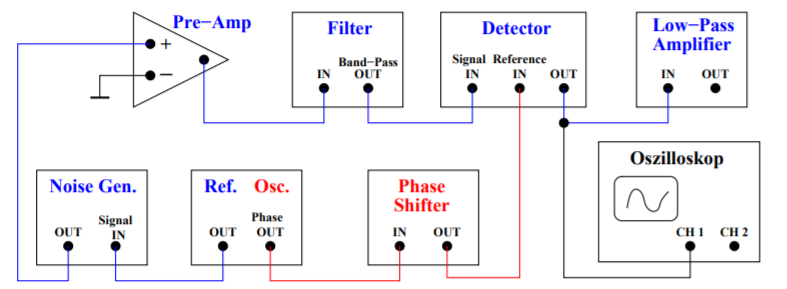
\includegraphics[width=\textwidth/2]{images/bild3.png}
    \caption{Schaltbild für einen Lock-In-Verstärker.\cite{V303}}
    \label{fig:bild3}
\end{figure}

$U_\text{sig}$ wird als sinusförmiges Signal verstärkt und zusammen mit einer sinusförmigen Referenzspannung auf den Mischer gegeben.
Es sind fünf verschiedene Phasen $\phi$ am Phase Shifter einzustellen und von den entstehenden Ausgaben des Oszilloskops wird jeweils ein Screenshot angefertigt.
Danach wird die Spannung $U_\text{out}$ nach dem Tiefpassfilter abgegriffen und auf dem Oszilloskop angezeigt.
$U_\text{out}$ wird für zehn verschiedene Phasen $\phi$ notiert.

Für die weiteren Messungen wird der Noice Generator in den Stromkreis eingebunden. 
Es werden zehn Phasenverschiebungen $\phi$ eingestellt.
Die Spannung $U_\text{out}$ wird erneut nach dem Tiefpassfilter abgegriffen und notiert.


Es wird eine Photodiodenschaltung nach \autoref{fig:bild4} aufgebaut.

\begin{figure}
    \centering
    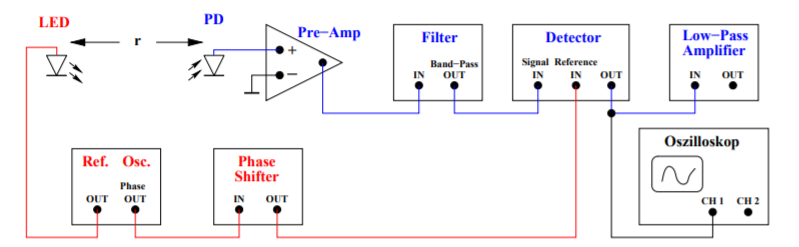
\includegraphics[width=\textwidth/2]{images/bild4.png}
    \caption{Schaltbild für einen Lock-In-Verstärker.\cite{V303}}
    \label{fig:bild4}
\end{figure}

Der Abstand $r$ zwischen der LED und der Photodiode, mit der das ausgesendete Licht gemessen wird, wird variiert.
Die Spannung $U_\text{out}$ wird in Abhängigkeit des Abstandes $r$ notiert.
Außerdem wird der maximale Abstand bestimmt, an dem die gemessene Spannung der Photodiode auf das Licht der LED zurückzuführen ist.